\chapter{Transverse waves}\fancyfoot[LO,RE]{Physics: Waves, Sound and Light}
    \setcounter{figure}{1}
    \setcounter{subfigure}{1}
    \label{m38806}
    \section{Introduction}
            \nopagebreak
%            \label{m38806*cid2} $ \hspace{-5pt}\begin{array}{cccccccccccc}   \end{array} $ \hspace{2 pt}\raisebox{-0.2em}{
\includegraphics[height=1em]{../icons/www.pdf}} {(section shortcode: P10040 )} \par 
      \label{m38806*id317331}Waves occur frequently in nature. The most obvious examples are
waves in water, on a dam, in the ocean, or in a bucket. We are
interested in the properties that waves have. All waves have
the same properties.

Waves do not only occur in water, they occur in any kind of medium. Earthquakes release enough energy to create waves that are powerful enough to travel through the rock of the Earth. When your friend speaks to you \textsl{sound waves} are produced that travel through the air to your ears. A wave is simply the disturbance of a medium by moving energy but how is it different from a pulse?.
\chapterstartvideo{VPgio}
    \section{What is a \textsl{transverse wave}?}

            \nopagebreak
%            \label{m38806*cid3} $ \hspace{-5pt}\begin{array}{cccccccccccc}   
\includegraphics[width=0.75cm]{col11305.imgs/summary_fullmarks.png} &   
\includegraphics[width=0.75cm]{col11305.imgs/summary_video.png} &   \end{array} $ \hspace{2 pt}\raisebox{-5 pt}{} {(section shortcode: P10041 )} \par 
\begin{minipage}{.5\textwidth}
\begin{center}
\textbf{Waves in a pool}\\
 \includegraphics[width=.8\textwidth]{photos/kreepykrawly.jpg}
\end{center}
\end{minipage}
\begin{minipage}{.5\textwidth}      
\label{m38806*id317690}We have studied pulses in \textit{Transverse pulses}, and know that a pulse is a single disturbance that travels through a medium. A \textsl{wave} is a periodic, continuous disturbance that consists of a \textsl{train} or \textsl{succession} of pulses.\par 
An enlarged version of the ripple tank can be seen in a real life example of a Kreepy Krauly\textregistered\ making waves in a pool because of the regular vibrations. The Kreepy Krauly\textregistered\ was invented in South Africa by Ferdinand Chauvier and his son Daniel.
\end{minipage}

\Definition{Wave}{A \textsl{wave} is a periodic, continuous disturbance that consists of a \textsl{train} of pulses.} 
\Definition{Transverse wave}{A \textsl{transverse wave} is a wave where the movement of the particles of the medium is perpendicular (at a right angle) to the direction of propagation of the wave.} 

\label{m38806*secfhsst!!!underscore!!!id89}
            \begin{activity}{Transverse waves }
            \nopagebreak
      \label{m38806*id317764}Take a rope or slinky spring. Have two people hold the rope or spring stretched out horizontally. Flick the one end of the rope up and down \textbf{continuously} to create a \textsl{train of pulses}.\par 
      \label{m38806*id317781}
    \setcounter{subfigure}{0}
	\begin{figure}[H] % horizontal\label{m38806*id317784}
    \begin{center}
\begin{pspicture}(0,-1.2546875)(7.62,1.2346874)
\psline[linewidth=0.04cm](1.6,0.5146875)(7.6,0.5146875)
\psline[linewidth=0.04cm](1.6,0.2146875)(7.6,0.2146875)
\psline[linewidth=0.02cm](1.64,0.5146875)(1.94,0.2146875)
\psline[linewidth=0.02cm](2.24,0.5146875)(2.54,0.2146875)
\psline[linewidth=0.02cm](2.84,0.5146875)(3.14,0.2146875)
\psline[linewidth=0.02cm](4.04,0.5146875)(4.34,0.2146875)
\psline[linewidth=0.02cm](3.44,0.5146875)(3.74,0.2146875)
\psline[linewidth=0.02cm](4.64,0.5146875)(4.94,0.2146875)
\psline[linewidth=0.02cm](5.24,0.5146875)(5.54,0.2146875)
\psline[linewidth=0.02cm](5.84,0.5146875)(6.14,0.2146875)
\psline[linewidth=0.02cm](6.44,0.5146875)(6.74,0.2146875)
\psline[linewidth=0.02cm](7.04,0.5146875)(7.34,0.2146875)
\psline[linewidth=0.04cm,arrowsize=0.1029cm 3.0,arrowlength=1.6,arrowinset=0.4]{<-}(1.2,-0.4853125)(1.2,1.2146875)
\psline[linewidth=0.04cm,arrowsize=0.1029cm 3.0,arrowlength=1.6,arrowinset=0.4]{->}(0.8,-0.4853125)(0.8,1.2146875)
\psline[linewidth=0.04cm,arrowsize=0.1029cm 3.0,arrowlength=1.6,arrowinset=0.4]{<-}(0.4,-0.4853125)(0.4,1.2146875)
\psline[linewidth=0.04cm,arrowsize=0.1029cm 3.0,arrowlength=1.6,arrowinset=0.4]{->}(0.0,-0.4853125)(0.0,1.2146875)
%\usefont{T1}{ptm}{m}{n}
\rput(2.1485937,-1.0353125){Flick rope up and down}
\end{pspicture}
\end{center}
 \end{figure}       
      \par 
      \label{m38806*id317791}\begin{enumerate}[noitemsep, label=\textbf{\arabic*}. ] 
            \label{m38806*uid1}\item Describe what happens to the rope.
\label{m38806*uid2}\item Draw a diagram of what the rope looks like while the pulses travel along it.
\label{m38806*uid3}\item In which direction do the pulses travel?
\label{m38806*uid4}\item Tie a ribbon to the middle of the rope. This indicates a particle in the rope.
    \setcounter{subfigure}{0}
	\begin{figure}[H] % horizontal\label{m38806*id317844}
   \begin{center}
\begin{pspicture}(0,-1.2446876)(7.64,1.2446876)
\psline[linewidth=0.04cm](1.62,0.5246875)(7.62,0.5246875)
\psline[linewidth=0.04cm](1.62,0.2246875)(7.62,0.2246875)
\psline[linewidth=0.02cm](1.66,0.5246875)(1.96,0.2246875)
\psline[linewidth=0.02cm](2.26,0.5246875)(2.56,0.2246875)
\psline[linewidth=0.02cm](2.86,0.5246875)(3.16,0.2246875)
\psline[linewidth=0.02cm](4.06,0.5246875)(4.36,0.2246875)
\psline[linewidth=0.02cm](3.46,0.5246875)(3.76,0.2246875)
\psline[linewidth=0.02cm](4.66,0.5246875)(4.96,0.2246875)
\psline[linewidth=0.02cm](5.26,0.5246875)(5.56,0.2246875)
\psline[linewidth=0.02cm](5.86,0.5246875)(6.16,0.2246875)
\psline[linewidth=0.02cm](6.46,0.5246875)(6.76,0.2246875)
\psline[linewidth=0.02cm](7.06,0.5246875)(7.36,0.2246875)
\psline[linewidth=0.04cm,arrowsize=0.1029cm 3.0,arrowlength=1.6,arrowinset=0.4]{<-}(1.22,-0.4753125)(1.22,1.2246875)
\psline[linewidth=0.04cm,arrowsize=0.1029cm 3.0,arrowlength=1.6,arrowinset=0.4]{->}(0.82,-0.4753125)(0.82,1.2246875)
\psline[linewidth=0.04cm,arrowsize=0.1029cm 3.0,arrowlength=1.6,arrowinset=0.4]{<-}(0.42,-0.4753125)(0.42,1.2246875)
\psline[linewidth=0.04cm,arrowsize=0.1029cm 3.0,arrowlength=1.6,arrowinset=0.4]{->}(0.02,-0.4753125)(0.02,1.2246875)
%\usefont{T1}{ptm}{m}{n}
\rput(2.1685936,-1.0253125){Flick rope up and down}
\psline[linewidth=0.08cm](4.52,0.5246875)(4.52,0.2246875)
\psbezier[linewidth=0.06](4.624195,0.5223207)(4.5021477,0.5799539)(4.558249,0.5731951)(4.604037,0.69499725)(4.649824,0.81679934)(4.7504873,0.9280784)(4.8152437,0.84101325)(4.88,0.75394803)(4.7462425,0.4646875)(4.624195,0.5223207)
\psline[linewidth=0.06cm](4.52,0.5446875)(4.84,0.1046875)
\psline[linewidth=0.06cm](4.5,0.4646875)(4.3,0.1246875)
\psbezier[linewidth=0.06](4.4578786,0.45692405)(4.6,0.50916064)(4.534671,0.5030347)(4.481353,0.6134316)(4.4280343,0.7238284)(4.3108144,0.8246875)(4.2354074,0.7457749)(4.16,0.6668623)(4.3157578,0.4046875)(4.4578786,0.45692405)
\end{pspicture}
\end{center}

 \end{figure}       \label{m38806*uid5}\item Flick the rope continuously. Watch the ribbon carefully as the pulses travel through the rope. What happens to the ribbon?
\label{m38806*uid6}\item Draw a picture to show the motion of the ribbon. Draw the ribbon as a dot and use arrows to indicate how it moves.
\end{enumerate}

\end{activity}

      \label{m38806*id317884}In the activity, you created waves. The medium through which these waves propagated was the rope, which is obviously made up of a very large number of particles (atoms).
From the activity, you would have noticed that the wave travelled from one side to the other, but the particles (the ribbon) moved only up and down.\par 
    \setcounter{subfigure}{0}
	\begin{figure}[H] % horizontal\label{m38806*uid7}
%    \begin{center}
%    \rule[.1in]{\figurerulewidth}{.005in} \\
%        \label{m38806*uid7!!!underscore!!!media}\label{m38806*uid7!!!underscore!!!printimage}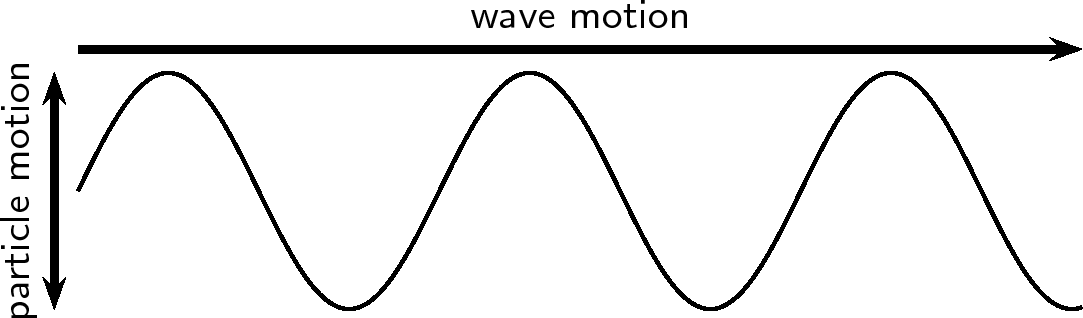
\includegraphics[width=300px]{col11305.imgs/m38806_PG10C5_003.png} % m38806;PG10C5\_003.png;;;6.0;8.5;
%      \vspace{2pt}
%    \vspace{\rubberspace}\par \begin{cnxcaption}
%	  \small \textbf{Figure 7.3: }A transverse wave, showing the direction of motion of the wave perpendicular to the direction in which the particles move.
%	\end{cnxcaption}
%    \vspace{.1in}
%    \rule[.1in]{\figurerulewidth}{.005in} \\
%    \end{center}
\begin{center}
\begin{pspicture}(-0.6,-1.6)(9,1.6)
%\psgrid
\psplot[xunit=0.017,plotpoints=300]{0}{500}{x 2 mul sin}
\psline[linewidth=2pt]{<->}(-0.2,-1)(-0.2,1)
\rput{90}(-0.5,0){particle motion}
\psline[linewidth=2pt]{->}(0,1.2)(8.5,1.2)
\uput[u](4.25,1.2){wave motion}
\end{pspicture}
\caption{A transverse wave, showing the direction of motion of the wave perpendicular to the direction in which the particles move.}
\label{m38806*uid7!!!underscore!!!media}
\end{center} 


\end{figure}       
      \label{m38806*id317903}When the particles of a medium move at right angles to the direction of propagation of a wave, the wave is called \textsl{transverse}. For waves, there is no net displacement of the particles of the medium (they return to their equilibrium position), but there is a net displacement of the wave. There are thus two different motions: the motion of the particles of the medium and the motion of the wave.\par 
      \label{m38806*eip-375}The following simulation will help you understand more about waves. Select the oscillate option and then observe what happens.
    \simulation{Phet simulation for Transverse Waves}{P10042}
 
            \section{Crests and troughs}
            \nopagebreak
        \label{m38806*id317923}Waves have moving \textsl{crests} (or \textsl{peaks}) and \textsl{troughs}. A crest is the highest point the medium rises to and a trough is the lowest point the medium sinks to.\par 
       crests and troughs on a transverse wave are shown in Figure~\ref{fig:p:wsl:tw10:transverse:peaktrough}.

\begin{figure}[htbp]
\begin{center}
\begin{pspicture}(-4,-1.1)(6,1.1)
%\psgrid
\psplot[xunit=0.0055,yunit=0.5,plotpoints=300]{-720}{720}{x sin }
\psline[linestyle=dashed](-4,0)(4,0)
\psline{<-}(4.1,0)(4.7,0)
\rput[l](4.8,0){equilibrium}
\rput[l](4.3,1){Crests}
\psline{<-}(-1.483,0.55)(-1.483,1)(3.5,1)
\psline{<-}(.497,0.55)(.497,1)(3.5,1)
\psline{<-}(2.477,0.55)(2.477,1)(3.5,1) \rput[l](4.3,-1){Troughs}
\psline{<-}(1.487,-0.55)(1.487,-1)(3.3,-1)
\psline{<-}(-.493,-0.55)(-.493,-1)(3.3,-1)
\psline{<-}(-2.473,-0.55)(-2.473,-1)(3.3,-1)
\end{pspicture}
\caption{Crests and troughs in a transverse wave.}
\label{fig:p:wsl:tw10:transverse:peaktrough}
\end{center}
\end{figure}
      
\par
\Definition{Crests and troughs} { \label{m38806*meaningfhsst!!!underscore!!!id136}
        \label{m38806*id317968}A \textsl{crest} is a point on the wave where the displacement of the medium is at a maximum. A point on the wave is a \textsl{trough} if the displacement of the medium at that point is at a minimum.  \par 
         } 
      \label{m38806*uid10}
\section{Amplitude}
\begin{activity}{Amplitude}
\begin{center}
\begin{pspicture}(-2,-1.4)(6,1.4)
%\psgrid
\def\halfwave{\psplot[xunit=0.0055,plotpoints=1200]{0}{1080}{x sin 1.4 mul}}
\rput(0,0){\halfwave\psline{<->}(0.5,0)(0.5,1.4)}
%\rput(0.7,0.875){a}
\psline[linestyle=dashed](0,0)(6,0)\uput[l](0,0){equilibrium}

\rput(0,0){\halfwave\psline{<->}(0.5,0)(0.5,1.4)\uput[r](0.4,0.6){a}}
\rput(2,0){%\rput[l]{180}{\halfwave}
\psline{<->}(-0.515,0)(-0.515,-1.4)\uput[r](-0.6,-0.6){b}}
\rput(2,0){%\halfwave
\psline{<->}(0.48,0)(0.48,1.4)\uput[r](0.4,0.6){c}}
\rput(4,0){%\rput[l]{180}{\halfwave}
\psline{<->}(-0.535,0)(-0.535,-1.4)\uput[r](-0.6,-0.6){d}}
\rput(4,0){%\halfwave
\psline{<->}(0.455,0)(0.455,1.4)\uput[r](0.4,0.6){e}}
\rput(6,0){%\rput[l]{180}{\halfwave}
\psline{<->}(-0.565,0)(-0.565,-1.4)\uput[r](-0.6,-0.6){f}}
\psline[linestyle=dashed](0,0)(6,0)\uput[l](0,0){equilibrium}
\end{pspicture}
\end{center}

Fill in the table below by measuring the distance between the equilibrium and each crest and trough in the wave above. Use your ruler to measure the distances.

\begin{center}
\begin{tabular}{|c|c|}\hline
Crest/Trough&Measurement (cm)\\\hline
a&\\\hline
b&\\\hline
c&\\\hline
d&\\\hline
e&\\\hline
f&\\\hline
\end{tabular}
\end{center}

\begin{enumerate}[noitemsep, label=\textbf{\arabic*}. ]
\item What can you say about your results?
\item Are the distances between the equilibrium position and each crest equal?
\item Are the distances between the equilibrium position and each trough equal?
\item Is the distance between the equilibrium position and crest equal to the distance between equilibrium and trough?
\end{enumerate}
\end{activity}

        \label{m38806*id318427}As we have seen in the activity on amplitude, the distance between the crest and the equilibrium position is equal to the distance between the trough and the equilibrium position. This distance is known as the \textsl{amplitude} of the wave, and is the characteristic height of the wave, above or below the equilibrium position. Normally the symbol $A$ is used to represent the amplitude of a wave. The SI unit of amplitude is the metre (m).
\Definition{Amplitude} {The amplitude of a wave is the maximum disturbance or displacement of the medium from the equilibrium (rest) position.\\
Quantity: Amplitude (A) \hspace{1cm} Unit name: metre \hspace{1cm} Unit symbol: $m$} 
        \label{m38806*id318448}
    \setcounter{subfigure}{0}
	\begin{figure}[H] % horizontal\label{m38806*id318451}
    \begin{center}
\begin{pspicture}(-5,-1)(5,1)%\psgrid
\psplot[xunit=0.0055,]{-360}{360}{x sin }
\psline[linestyle=dashed](-3,0)(3,0)
\rput(4,0.5){Amplitude}
\psline{<->}(3.,0)(3.,1)
\rput(4,-.5){Amplitude}
\psline{<->}(3.,0)(3.,-1)
\psline[linestyle=dashed](.495,1)(3,1)
\psline[linestyle=dashed](1.485,-1)(3,-1)
\psline{<->}(-3,-1)(-3,1)
\rput(-4.5,0){2 x Amplitude}
\end{pspicture}
\end{center}
 \end{figure}       
        \par 
\label{m38806*secfhsst!!!underscore!!!id212}

\IFact{
A tsunami is a series of sea waves caused by an underwater earthquake, landslide, or volcanic eruption. When the ocean is deep, tsunamis may be less than a 30~cm high on the ocean's€™s surface and can travel at speeds up to 700~$\text{km}\cdot \text{hr}^{-1}$.
In shallow water near the coast, it slows down. The top of the wave moves faster than the bottom, causing the sea to rise dramatically, as much as 30 m.
The wavelength can be as long as 100 km and the period as long as a hour.

In 2004, the Indian Ocean tsunami was caused by an earthquake that is thought to have had the energy of 23,000 atomic bombs. Within hours of the earthquake, killer waves radiating from away from the earthquake crashed into the coastline of 11 countries, killing 150,000 people. The final death toll was 283,000.
}

\begin{wex}{Amplitude of sea waves}{If the crest of a wave measures $2~\text{m}$ above the still water mark in the harbour, what is the amplitude of the wave?}{%solution
\westep{Analyse the information provided}{
We have been told that the harbour has a still water mark. This is a line created when there are no disturbances in the water, which means that it is the equilibrium position of the water.
}
\westep{Determine the amplitude}{  
        \label{m38806*id318492}The definition of the amplitude is the height of a crest above the equilibrium position. The still water mark is the height of the water at equilibrium and the crest is $2\phantom{\rule{2pt}{0ex}}\text{m}$ above this, so the amplitude is $2\phantom{\rule{2pt}{0ex}}\text{m}$.
}
}
\end{wex}
    

\noindent
\label{m38806*secfhsst!!!underscore!!!id221}
            \begin{activity}{Wavelength}
            \nopagebreak
      

\begin{figure}[H] % horizontal\label{m38806*id318520}
    \begin{center}
\begin{pspicture}(-2,-2.6)(6,2.6)
%\psgrid%[gridcolor=lightgray]
\psplot[xunit=0.00555556,plotpoints=300]{0}{1080}{x sin 1.8 mul}
\pcline[offset=-8pt]{|-|}(1.5,-1.8)(3.5,-1.8)
\bput{:U}{a}
\pcline[offset=-8pt]{|-|}(3.5,-1.8)(5.5,-1.8)
\bput{:U}{b}
\pcline[offset=8pt]{|-|}(0.5,1.8)(2.5,1.8)
\aput{:U}{c}
\pcline[offset=8pt]{|-|}(2.5,1.8)(4.5,1.8)
\aput{:U}{d}
\psline[linestyle=dashed](0,0)(6,0)\uput[l](0,0){equilibrium}
\end{pspicture}
\end{center} \end{figure}       
        
        \label{m38806*id318526}Fill in the table below by measuring the distance between crests and troughs in the wave above.\par 
    % \textbf{m38806*id318530}\par
\begin{center}
\begin{tabular}{|c|c|}\hline
&Distance(cm)\\\hline
a&\\\hline
b&\\\hline
c&\\\hline
d&\\\hline
\end{tabular}
\end{center}
    \par
        \label{m38806*id318631}\begin{enumerate}[noitemsep, label=\textbf{\arabic*}. ] 
            \label{m38806*uid15}\item What can you say about your results?
\label{m38806*uid16}\item Are the distances between crests equal?
\label{m38806*uid17}\item Are the distances between troughs equal?
\label{m38806*uid18}\item Is the distance between crests equal to the distance between troughs?
\end{enumerate}

\end{activity}

        \label{m38806*id318690}As we have seen in the activity on wavelength, the distance between two \textsl{adjacent} crests is the same no matter which two adjacent crests you choose. There is a fixed distance between the crests. Similarly, we have seen that there is a fixed distance between the troughs, no matter which two troughs you look at. More importantly, the distance between two adjacent crests is the same as the distance between two adjacent troughs. This distance is called the \textsl{wavelength} of the wave.\par 
        \label{m38806*id318708}The symbol for the wavelength is $\lambda $ (the Greek letter \textsl{lambda}) and wavelength is measured in metres ($\text{m}$).\par 
        \label{m38806*id318725}
    \setcounter{subfigure}{0}
	\begin{figure}[H] % horizontal\label{m38806*id318728}
   \begin{center}
\begin{pspicture}(-2,-1.1)(2,1.1)
%\psgrid
\psplot[xunit=0.0055,]{-360}{360}{x sin}
\psline[linestyle=dashed](-3,0)(3,0)
\rput(-.5,1.35){$\lambda$}
\psline{<->}(0.495,1.06)(-1.485,1.06)
\rput(0.5,-1.35){$\lambda$}
\psline{<->}(-0.495,-1.06)(1.485,-1.06)
\end{pspicture}
\end{center} \end{figure}       
        \par 


\begin{wex}{Wavelength}{The total distance between 4 consecutive crests of a transverse wave is 6\,m. What is the wavelength of the wave?}{
\westep{Draw a rough sketch of the situation}

\begin{center}
\begin{pspicture}(-2,-2)(8,2.6)
%\psgrid%[gridcolor=lightgray]
\psplot[xunit=0.00555556,plotpoints=300]{0}{1440}{x sin 1.8 mul}
\pcline[offset=16pt]{|-|}(0.5,1.8)(6.5,1.8)
\aput{:U}{6\,m}
\psline[linestyle=dashed](0,0)(8,0)\uput[l](0,0){equilibrium}
\pcline[offset=8pt]{|-|}(0.5,1.8)(2.5,1.8)
\bput{:U}{$\lambda$}
\pcline[offset=8pt]{-|}(2.5,1.8)(4.5,1.8)
\bput{:U}{$\lambda$}
\pcline[offset=8pt]{-|}(4.5,1.8)(6.5,1.8)
\bput{:U}{$\lambda$}

\end{pspicture}
\end{center}

\westep{Determine how to approach the problem}
From the sketch we see that 4 consecutive crests is equivalent to 3 wavelengths.

\westep{Solve the problem}
Therefore, the wavelength of the wave is:
\begin{eqnarray*}
3\lambda&=&6~\text{m}\\
\lambda&=&\frac{6~\text{m}}{3}\\
&=&2\,\text{m}
\end{eqnarray*}
\westep{Quote the final answer}
The wavelength is 2~m.
}
\end{wex}


\section{Points in phase}
            \nopagebreak
\label{m38806*secfhsst!!!underscore!!!id359}
\begin{activity}{Points in phase}

Fill in the table by measuring the distance between the indicated points.

\begin{center}
\begin{pspicture}(0,-2)(5.4,2.4)
\psgrid[gridcolor=lightgray,gridlabels=0]
\psset{xunit=0.0075}
\psplot[plotpoints=300]{0}{720}{x sin 1.8 mul}
\pnode(!0 0 sin 1.8 mul){a}
\pnode(!20 20 sin 1.8 mul){b}
\pnode(!60 60 sin 1.8 mul){c}
\pnode(!90 90 sin 1.8 mul){d}
\pnode(!180 180 sin 1.8 mul){e}
\pnode(!360 360 sin 1.8 mul){f}
\pnode(!380 380 sin 1.8 mul){g}
\pnode(!420 420 sin 1.8 mul){h}
\pnode(!450 450 sin 1.8 mul){i}
\pnode(!540 540 sin 1.8 mul){j}

\psdot(a)\uput[l](a){A}
\psdot(b)\uput[l](b){B}
\psdot(c)\uput[l](c){C}
\psdot(d)\uput[u](d){D}
\psdot(e)\uput[l](e){E}
\psdot(f)\uput[l](f){F}
\psdot(g)\uput[l](g){G}
\psdot(h)\uput[l](h){H}
\psdot(i)\uput[u](i){I}
\psdot(j)\uput[d](j){J}
\end{pspicture}
\end{center}

\begin{center}
\begin{tabular}{|c|c|}\hline
\textbf{Points} & \textbf{Distance (cm)}\\\hline\hline
A to F&\\\hline
B to G&\\\hline
C to H&\\\hline
D to I&\\\hline
E to J&\\\hline

\hline
\end{tabular}
\end{center}

What do you find?

\end{activity}

   \label{m38806*id319071}In the activity the distance between the indicated points was equal. These points are then said to be \textsl{in phase}. Two points in phase are separate by an whole (1,2,3,...) number multiple of  whole wave cycles or wavelengths. The points in phase do not have to be crests or troughs, but they must be separated by a complete number of wavelengths.\par 
        \label{m38806*id319082}We then have an alternate definition of the wavelength as the distance between any two adjacent points which are \textsl{in phase}.\par 


\Definition{Wavelength of wave } { \label{m38806*meaningfhsst!!!underscore!!!id408}
        \label{m38806*id319098}The wavelength of a wave is the distance between any two adjacent points that are in phase. \par 
         } 
        

\label{m38806*id319111}
    \setcounter{subfigure}{0}
	\begin{figure}[H] % horizontal\label{m38806*id319114}
    \begin{center}
\begin{pspicture}(-3,-1.5)(3,1.5)
%\psgrid
\psplot[xunit=0.0055,]{-360}{360}{x sin}
\psline[linestyle=dashed](-3,0)(3,0)
\pcline[offset=0pt]{<->}(-1.485,1.06)(0.495,1.06)
\aput{:U}{$\lambda$}
\pcline[offset=0pt]{<->}(-0.495,-1.06)(1.485,-1.06)
\bput{:U}{$\lambda$}
\pcline{<->}(-1,0)(1,0)
\lput*{:U}{$\lambda$}
\pcline{<->}(-1.83,0.5)(0.167,0.5)
\lput*{:U}{$\lambda$}
\end{pspicture}
\end{center}

 \end{figure}       
        \par 
        \label{m38806*id319121}Points that are not in phase, those that are not separated by a complete number of wavelengths, are called \textsl{out of phase}. Examples of points like these would be $A$ and $C$, or $D$ and $E$, or $B$ and $H$ in the Activity.\par 
      \label{m38806*uid20}
            \section{Period and frequency}
            \nopagebreak
        \label{m38806*id319195}Imagine you are sitting next to a pond and you watch the waves going past you. First one crest arrives, then a trough, and then another crest. Suppose you measure the time taken between one crest arriving and then the next. This time will be the same for any two successive crests passing you. We call this
time the \textsl{period}, and it is a characteristic of the wave.\par 
        \label{m38806*id319207}The symbol $T$ is used to represent the period. The period is measured in seconds ($\text{s}$).\par 

\Definition{Period} { \label{m38806*meaningfhsst!!!underscore!!!id426}The period is the time taken for two successive crests (or troughs) to pass a fixed point.\\
Quantity: Period ($T$) \hspace{1cm} Unit name: second \hspace{1cm} Unit symbol: s  } 


\label{m38806*id319238}Imagine the pond again. Just as a crest passes you, you start your stopwatch and count each crest going past. After 1 second you stop the clock and stop counting. The number of crests that you have counted in the 1 second is the \textsl{frequency} of the wave.\par 

\Definition{Frequency } { The frequency is the number of successive crests (or troughs) passing a given point in 1 second.\\
Quantity: Frequency ($f$) \hspace{1cm} Unit name: hertz \hspace{1cm} Unit symbol: Hz } 
        
The frequency and the period are related to each other. As the period is the time taken for 1 crest to pass, then the number of crests passing the point in 1 second is $\frac{1}{T}$. But this is the frequency. So
\begin{equation*}
\boxed{f=\frac{1}{T}}
\end{equation*}
or alternatively,
\begin{equation*}
\boxed{T=\frac{1}{f}}.
\end{equation*}

For example, if the time between two consecutive crests passing a fixed point is $\frac{1}{2}\,$s, then the period of the wave is $\frac{1}{2}\,$s. Therefore, the frequency of the wave is:
\begin{eqnarray*}
f&=&\frac{1}{T}\\
&=&\frac{1}{\frac{1}{2}\es}\\
&=&2 \text{ s}^{-1}
\end{eqnarray*}
The unit of frequency is the Hertz (Hz) or $\text{s}^{-1}$.
\pagebreak

\begin{wex}{Period and frequency}{What is the period of a wave of frequency 10\,Hz?}{
\westep{Determine what is given and what is required}
We are required to calculate the period of a 10\,Hz wave.

\westep{Determine how to approach the problem}
We know that:
\begin{equation}
T=\frac{1}{f}\nonumber 
\end{equation}

\westep{Solve the problem}\begin{eqnarray*}
T&=&\frac{1}{f}\\
&=&\frac{1}{10\,\text{Hz}}\\
&=&0,1\,\text{s}
\end{eqnarray*}
\westep{Write the answer}
The period of a 10\,Hz wave is 0,1\,s.}
\end{wex}

    \noindent
      \label{m38806*uid21}
            \section{Speed of a transverse wave}
            \nopagebreak
       \Definition{Wave speed }{Wave speed is the distance a wave travels per unit time.\\
	  Quantity: Wave speed ($v$) \hspace{1cm} Unit name: metre per second \hspace{1cm} Unit symbol: $\text{m}\cdot \text{s}^{-1}$
         } 
   
        \label{m38806*id319706}The distance between two successive crests is 1 wavelength, $\lambda $. Thus in a time of 1 period, the wave will travel 1 wavelength in distance. Thus the speed of the wave, $v$, is:\par 
        \label{m38806*id319732}\nopagebreak\noindent{}
    \begin{equation}\nonumber
    \boxed{v=\frac{\text{distance}\phantom{\rule{4.pt}{0ex}}\text{travelled}}{\text{time}\phantom{\rule{4.pt}{0ex}}\text{taken}}=\frac{\lambda }{T}}
      \end{equation}
        \label{m38806*id319776}However, $f=\frac{1}{T}$. Therefore, we can also write:\par 
        \label{m38806*id319802}\nopagebreak\noindent{}
          
    \begin{equation}\nonumber
    \begin{array}{ccc}\hfill v& =& \frac{\lambda }{T}\hfill \\ & =& \lambda \ensuremath{\cdot}\frac{1}{T}\hfill \\ & =& \lambda \ensuremath{\cdot}f\hfill \end{array}
      \end{equation}
        \label{m38806*id319870}We call this equation the \textsl{wave equation}. To summarise, we have that $v=\lambda \ensuremath{\cdot}f$ where\par 
        \label{m38806*id319901}\begin{itemize}[noitemsep]
            \label{m38806*uid22}\item $v=$ speed in $\text{m}\ensuremath{\cdot}\text{s}{}^{-1}$\label{m38806*uid23}\item $\lambda =$ wavelength in $\text{m}$
\label{m38806*uid24}\item $f=$ frequency in $\text{Hz}$
\end{itemize}

\subsubsection{Wave equation}
\begin{equation*}\nonumber
    \boxed{v = f\cdot \lambda}\hspace{1cm}\text{or}\hspace{1cm} \boxed{v = \frac{\lambda }{T}}
      \end{equation*}

\begin{wex}{Speed of a transverse wave I}{When a particular string is vibrated at a frequency of 10\,Hz, a transverse wave of wavelength 0,25\,m is produced. Determine the speed of the wave as it travels along the string.}
{\westep{Determine what is given and what is required}
\begin{itemize}
\item{frequency of wave: $f=$\,10\,Hz}
\item{wavelength of wave: $\lambda=$\,0,25\,m}
\end{itemize}
We are required to calculate the speed of the wave as it travels along the string. All quantities are in SI units.

\westep{Determine how to approach the problem}
We know that the speed of a wave is:
\begin{equation*}
v=f\cdot \lambda 
\end{equation*}
and we are given all the necessary quantities.

\westep{Substituting in the values}
\begin{eqnarray*}
v&=&f\cdot \lambda\\
&=&(10\;\text{Hz})(0,25~\text{m})\\
&=&(10\;\text{s}^{-1})(0,25~\text{m})\\
&=&2,5~\text{m} \cdot \text{s}^{-1}
\end{eqnarray*}

\westep{Write the final answer}
The wave travels at 2,5\,\ms\ along the string.
}
\end{wex}


\begin{wex}{Speed of a transverse wave II}{A cork on the surface of a swimming pool bobs up and down once every second on some ripples. The ripples have a wavelength of 20\,cm. If the cork is 2\,m from the edge of the pool, how long does it take a ripple passing the cork to reach the edge?}{
\westep{Determine what is given and what is required}
We are given:
\begin{itemize}
\item{frequency of wave: $f =$ 1\,Hz}
\item{wavelength of wave: $\lambda =$ 20\,cm}
\item{distance of cork from edge of pool: $D\,=$ 2\,m}
\end{itemize}
We are required to determine the time it takes for a ripple to travel between the cork and the edge of the pool.

The wavelength is not in SI units and should be converted.

\westep{Determine how to approach the problem}
The time taken for the ripple to reach the edge of the pool is obtained from:
$$t=\frac{D}{v} \ \ \ \ \ (\text{from}\ v=\frac{D}{t})$$
We know that
\begin{equation*}v=f\cdot \lambda\end{equation*}
Therefore,
\begin{equation}t=\frac{D}{f\cdot \lambda}\end{equation}

\westep{Convert wavelength to SI units}
\begin{equation*}20\,\text{cm}=0,2\,\text{m}\end{equation*}

\westep{Solve the problem}
\begin{eqnarray*}
t&=&\frac{d}{f\cdot \lambda}\\
&=&\frac{2~\text{m}}{(1\;\text{Hz})(0,2~\text{m})}\\
&=&\frac{2~\text{m}}{(1\;\text{s}^{-1})(0,2~\text{m})}\\
&=&10\ \text{s}
\end{eqnarray*}
\westep{Write the final answer}
A ripple passing the leaf will take 10\,s to reach the edge of the pool.}
\end{wex}

    \mindsetvid{Video on waves}{VPcci}
            \begin{exercises}{Waves}
            \nopagebreak\vspace{-1cm}
            \label{m38806*id320717}\begin{enumerate}[noitemsep, label=\textbf{\arabic*}. ] 
            \label{m38806*uid30}\item When the particles of a medium move perpendicular to the direction of the wave motion, the wave is called a $.........$ wave.\newline
\label{m38806*uid31}\item A transverse wave is moving downwards. In what direction do the particles in the medium move?\newline
\label{m38806*uid32}\item Consider the diagram below and answer the questions that follow:
    \setcounter{subfigure}{0}
	\begin{figure}[H] % horizontal\label{m38806*id320776}
    \begin{center}
\begin{pspicture}(0,-1)(8,1)
%\psgrid[gridcolor=lightgray]
\psset{xunit=0.01111}
\psline(0,0)(720,0)
\psplot{0}{720}{x sin}
\pcline{<->}(90,-1)(90,1)
\lput*{:U}{A}
\pcline{<->}(450,0)(450,1)
\lput*{:U}{B}
\pcline{<->}(90,-1)(270,-1)
\lput*{:U}{C}
\pcline{<->}(270,-1)(630,-1)
\lput*{:U}{D}
\psline(270,-1.2)(270,-0.8)
\end{pspicture}
\end{center}
 \end{figure}       \label{m38806*id320783}\begin{enumerate}[noitemsep, label=\textbf{\alph*}. ] 
            \label{m38806*uid33}\item the wavelength of the wave is shown by letter \uline{\hspace{10ex}}.
\label{m38806*uid34}\item the amplitude of the wave is shown by letter \uline{\hspace{10ex}}.
\end{enumerate}
                \label{m38806*uid35}\item Draw 2 wavelengths of the following transverse waves on the same graph paper. Label all important values.
\label{m38806*id320849}\begin{enumerate}[noitemsep, label=\textbf{\alph*}. ] 
            \label{m38806*uid36}\item Wave 1: Amplitude = 1~cm, wavelength = 3~cm
\label{m38806*uid37}\item Wave 2: Peak to trough distance (vertical) = 3~cm, crest to crest distance (horizontal) = 5~cm
\end{enumerate}
                \label{m38806*uid38}\item You are given the transverse wave below.
    \setcounter{subfigure}{0}
	\begin{figure}[H] % horizontal\label{m38806*id320895}
    \begin{center}
\begin{pspicture}(-0.6,-1.2)(4.2,1.2)
%\psgrid[gridcolor=gray]
\psaxes{<->}(0,0)(0,-1.2)(4.2,1.2)
\psplot[xunit=0.005573]{0}{720}{x sin}
\end{pspicture}
\end{center}

 \end{figure}       
Draw the following:
\label{m38806*id320905}\begin{enumerate}[noitemsep, label=\textbf{\alph*}. ] 
            \label{m38806*uid39}\item A wave with twice the amplitude of the given wave.
\label{m38806*uid40}\item A wave with half the amplitude of the given wave.
\label{m38806*uid41}\item A wave travelling at the same speed with twice the frequency of the given wave.
\label{m38806*uid42}\item A wave travelling at the same speed with half the frequency of the given wave.
\label{m38806*uid43}\item A wave with twice the wavelength of the given wave.
\label{m38806*uid44}\item A wave with half the wavelength of the given wave.
\label{m38806*uid45}\item A wave travelling at the same speed with twice the period of the given wave.
\label{m38806*uid46}\item A wave travelling at the same speed with half the period of the given wave.
\end{enumerate}
                \label{m38806*uid47}\item A transverse wave travelling at the same speed with an amplitude of 5~cm has a frequency of 15~Hz. The horizontal distance from a crest to the nearest trough is measured to be 2,5~cm. Find the
\label{m38806*id321026}\begin{enumerate}[noitemsep, label=\textbf{\alph*}. ] 
            \label{m38806*uid48}\item period of the wave.
\label{m38806*uid49}\item speed of the wave.
\end{enumerate}
                \label{m38806*uid50}\item A fly flaps its wings back and forth 200 times each second. Calculate the period of a wing flap.\newline
\label{m38806*uid51}\item As the period of a wave increases, the frequency 
\textsl{\textbf{increases/decreases/does not change.}}\newline
\label{m38806*uid52}\item Calculate the frequency of rotation of the second hand on a clock.\newline
\label{m38806*uid53}\item Microwave ovens produce radiation with a frequency of 2 450~MHz (1~MHz = ${10}^{6}$~Hz) and a wavelength of 0,122~m. What is the wave speed of the radiation?\newline
\label{m38806*uid54}\item Study the following diagram and answer the questions:
    \setcounter{subfigure}{0}
	\begin{figure}[H] % horizontal\label{m38806*id321151}
    \begin{center}
\begin{pspicture*}(-0.6,-1.6)(4.6,1.6)
\psgrid[gridcolor=lightgray]
\psset{xunit=0.0055}
\psplot{0}{720}{x sin}
\pnode(!0 0 sin){a}
\pnode(!45 45 sin){b}
\pnode(!90 90 sin){c}
\pnode(!135 135 sin){d}
\pnode(!180 180 sin){e}
\pnode(!225 225 sin){f}
\pnode(!270 270 sin){g}
\pnode(!315 315 sin){h}
\pnode(!360 360 sin){i}
\pnode(!405 405 sin){j}
\pnode(!450 450 sin){k}
\pnode(!495 495 sin){l}
\pnode(!540 540 sin){m}
\pnode(!585 585 sin){n}
\pnode(!630 630 sin){o}
\pnode(!675 675 sin){p}
\pnode(!720 720 sin){q}

\psdot(a)\uput[l](a){A}
\psdot(b)\uput[l](b){B}
\psdot(c)\uput[u](c){C}
\psdot(d)\uput[r](d){D}
\psdot(e)\uput[r](e){E}
\psdot(f)\uput[l](f){F}
\psdot(g)\uput[d](g){G}
\psdot(h)\uput[r](h){H}
\psdot(i)\uput[l](i){I}
\psdot(j)\uput[l](j){J}
\psdot(k)\uput[u](k){K}
\psdot(l)\uput[r](l){L}
\psdot(m)\uput[r](m){M}
\psdot(n)\uput[l](n){N}
\psdot(o)\uput[d](o){O}
\psdot(p)\uput[r](p){P}
\psdot(q)\uput[r](q){Q}
\end{pspicture*}
\end{center}

 \end{figure}       \label{m38806*id321157}\begin{enumerate}[noitemsep, label=\textbf{\alph*}. ] 
            \label{m38806*uid55}\item Identify two sets of points that are in phase.
\label{m38806*uid56}\item Identify two sets of points that are out of phase.
\label{m38806*uid57}\item Identify any two points that would indicate a wavelength.
\end{enumerate}
                \label{m38806*uid58}\item Tom is fishing from a pier and notices that four wave crests pass by in 8~s and estimates the distance between two successive crests is 4~m. The timing starts with the first crest and ends with the fourth. Calculate the speed of the wave.\newline
\end{enumerate}
\par \practiceinfo
 \par \begin{tabular}[h]{cccccc}
 (1.) 0039  &  (2.) 003a  &  (3.) 003b  &  (4.) 003c  &  (5.) 003d  &  (6.) 003e  &  (7.) 003f  &  (8.) 003g  &  (9.) 003h  &  (10.) 003i  &  (11.) 003j  &  (12.) 003k  & \end{tabular}

\end{exercises}    

\summary{VPguj}
            \nopagebreak
%            \label{m38806*cid6} $ \hspace{-5pt}\begin{array}{cccccccccccc}   \end{array} $ \hspace{2 pt}\raisebox{-0.2em}{
\includegraphics[height=1em]{../icons/www.pdf}} {(section shortcode: P10044 )} \par 
      \label{m38806*id324089}\begin{itemize}[noitemsep] 
            \label{m38806*uid108}\item A wave is formed when a continuous number of pulses are transmitted through a medium.
\label{m38806*uid109}\item A crest is the highest point a particle in the medium rises to.
\label{m38806*uid110}\item A trough is the lowest point a particle in the medium sinks to.
\label{m38806*uid111}\item In a transverse wave, the particles move perpendicular to the motion of the wave.
\label{m38806*uid112}\item The amplitude ($A$) is the maximum distance from equilibrium position to a crest (or trough), or the maximum displacement of a particle in a wave from its position of rest.
\label{m38806*uid113}\item The wavelength ($\lambda $) is the distance between any two adjacent points on a wave that are in phase. It is measured in metres.
\label{m38806*uid114}\item The period ($T$) of a wave is the time it takes a wavelength to pass a fixed point. It is measured in seconds (s).
\label{m38806*uid115}\item The frequency ($f$) of a wave is how many waves pass a point in a second. It is measured in hertz (Hz) or $\text{s}{}^{-1}$.
\label{m38806*uid116}\item Frequency: $f=\frac{1}{T}$\label{m38806*uid117}\item Period: $T=\frac{1}{f}$\label{m38806*uid118}\item Speed: $v=f\cdot\lambda $ or $v=\frac{\lambda }{T}$.
\end{itemize}

%\begin{table}[H]
%\begin{center}
%\begin{tabular}{|l|c|c|c|}\hline \hline 
%\multicolumn{4}{|c|}{\textbf{Units}}\\ \hline \hline
%\textbf{Quantity} & \textbf{Symbol} & \textbf{Unit} & \textbf{S.I. Units}\\ \hline
%Amplitude & $A$ & \multicolumn{2}{c|}{m} \\ \hline
%Wavelength & $\lambda$ & \multicolumn{2}{c|}{m}  \\ \hline
%Period & $T$ & \multicolumn{2}{c|}{s}  \\ \hline
%Frequency & $f$ & \multicolumn{2}{c|}{$\text{s}^{-1}$}  \\ \hline
%Wave speed & $v$ & \multicolumn{2}{c|}{$\text{m} \cdot \text{s}^{-1}$} \\ \hline
%\end{tabular}
%\end{center}
%\caption{Units used in \textbf{transverse waves} }
%\label{table:electricity::units}
%\end{table}

\begin{table}[H]
\begin{center}
\begin{tabular}{|l|c|c|}\hline \hline 
\multicolumn{3}{|c|}{\textbf{Physical Quantities}}\\ \hline \hline
\multicolumn{1}{|c|}{\textbf{Quantity}} & \textbf{Unit name} & \textbf{Unit symbol}\\ \hline
Amplitude ($A$) & metre & m \\ \hline
Wavelength ($\lambda$) & metre & m \\ \hline
Period ($T$) & second & s \\ \hline
Frequency ($f$) & hertz & Hz \ \ ($s^{-1}$) \\ \hline
Wave speed ($v$) & metre per second & $\text{m} \cdot \text{s}^{-1}$ \\ \hline
\end{tabular}
\end{center}
\caption{Units used in \textbf{transverse waves} }
\label{table:electrostatics::units}
\end{table}






    \begin{eocexercises}{Waves}
            \nopagebreak
%            \label{m38806*cid7} $ \hspace{-5pt}\begin{array}{cccccccccccc}   \end{array} $ \hspace{2 pt}\raisebox{-0.2em}{
\includegraphics[height=1em]{../icons/www.pdf}} {(section shortcode: P10045 )} \par 
      \label{m38806*id324367}\begin{enumerate}[noitemsep, label=\textbf{\arabic*}. ] 
\label{m38806*uid128}\item A wave travels along a string at a speed of $1,5\text{m}\ensuremath{\cdot}\text{s}{}^{-1}$. If the frequency of the source of the wave is 7,5 Hz, calculate:
\label{m38806*id324525}\begin{enumerate}[noitemsep, label=\textbf{\alph*}. ] 
            \label{m38806*uid129}\item the wavelength of the wave
\label{m38806*uid130}\item the period of the wave
\end{enumerate}
                \item Water waves crash against a seawall around the harbour. Eight waves hit the seawall in 5 s. The distance between successive troughs is 9 m. The height of the waveform trough to crest is 1,5 m. 
    \setcounter{subfigure}{0}
	\begin{figure}[H] % horizontal\label{m38806*id634524}
    \begin{center}
    \label{m38806*id634524!!!underscore!!!media}\label{m38806*id634524!!!underscore!!!printimage}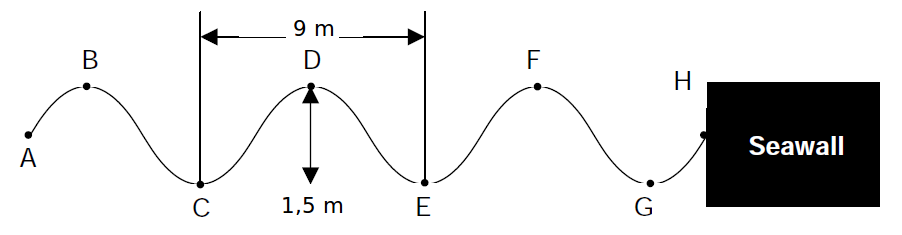
\includegraphics[width=0.8\columnwidth]{col11305.imgs/m38806_seawall.png} % m38806;seawall.png;;;6.0;8.5;
    \end{center}
 \end{figure}       
\label{m38806*uid081231}\begin{enumerate}[noitemsep, label=\textbf{\alph*}. ] 
            \item How many complete waves are indicated in the sketch?\item Write down the letters that indicate any TWO points that are:
\label{m38806*uid0821323}\begin{enumerate}[noitemsep, label=\textbf{\roman*}. ] 
            \item in phase\item out of phase\item Represent ONE wavelength.\end{enumerate}
        \item Calculate the amplitude of the wave.\item Show that the period of the wave is 0,67 s.\item Calculate the frequency of the waves.\item Calculate the velocity of the waves.\end{enumerate}
         \end{enumerate}
  \label{m38806**end}
\par \practiceinfo
 \par \begin{tabular}[h]{cc}
(1.) 003m  &  (2.) 003n  & \end{tabular}

\end{eocexercises}
